\section{Problema 2: Reconfiguraci\'on de rutas}

\subsection{Introducci\'on}

\quad Se desea optimizar las conexiones existentes entre un conjunto de ciudades. Se pueden construir nuevos caminos o destruir existentes. Ambas operaciones tienen un costo asociado. Se desea optimizar gastando la menor cantidad de dinero posible. Solo puede haber una forma de ir de una ciudad a otra y no existen varias rutas entre dos mismas ciudades. Bajo estas premisas resolvimos el problema como detallaremos a continuación.


\subsection{Desarrollo}

\quad Decidimos modelar el problema con grafos. Donde, los nodos son las ciudades y las aristas son las rutas existentes y las posibles a construir. Cada eje tiene un costo asociado, ya sea para destruir o construir la ruta que simboliza. Destacamos el hecho de que las instancias del problema por consigna tienen $ \frac{n * (n - 1)}{2} $ aristas donde $ n $ es la cantidad de ciudades. Por la propiedad de grafos vista en la cursada, esa es la cantidad de aristas que tienen los grafos completos de $ n $ nodos.

\quad

\quad Luego, utilizamos el algoritmo modificado de Kruskal para generar un \'arbol generador m\'inimo (AGM) del grafo. A diferencia de realizar normalmente este algoritmo, utilizamos un ordenamiento de las aristas distinto. Primero consideramos como menores todas las aristas de rutas ya construidas que las no existentes. Luegos, las existentes las ordenamos de mayor a menor según el valor asociado. En cambio, las no construidas las ordenamos de menor a mayor. En la parte de correctitud explicaremos el motivo de tal ordenamiento. Podemos resolver el problema con un AGM pues cada ruta es doble vía, se quiere que todas las ciudades est\'en conectadas y que haya una sola forma de ir de una ciudad a otra.

\quad Para generar el AGM utilizamos una estructuras de datos llamada \textit{Find Union Set} o \textit{Disjoint Set} \footnote{UnionFind Set, Introduction to Algorithms 2nd Edition, Capitulo 21. Autores: Thomas H. Cormen, Charles E. Leiserson, Ronald L, Rivest, Clifford Stein} . Nos permite tener informaci\'on de elementos particionados en clases de equivalencia. Es decir, podemos manejar particiones disjuntas de un conjunto. En este caso, el conjunto de nodos. Las particiones ser\'ian los nodos que pertenecen a una componente conexa. La relaci\'on de clase de equivalencia ser\'ia que exista un camino entre los elementos (nodos) de la clase. En el algoritmo de Kruskal, nos permite determinar si se agregase cierta arista se forma o no un ciclo.

\quad 


\begin{figure}[H]
	\centering
	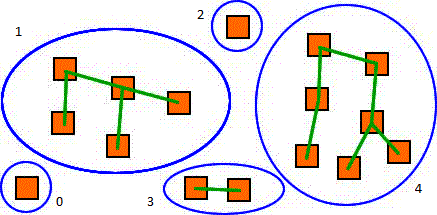
\includegraphics[scale=0.8]{DisjointSets.png}
\caption{Disjoint Set donde hay 5 clases de equivalencia. Los cuadrados naranjas representan nodos y las l\'ineas verdes aristas. Se observa que la relaci\'on es que est\'en en la misma componente conexa.}
\end{figure}



\quad Una vez obtenido el AGM, para calcular el costo de la optimizaci\'on de la conectividad entre las ciudades, es cuesti\'on de recorrer el AGM primero fijándose las aristas que est\'an presentes. Si son aristas de rutas ya existentes no aportan al costo, y si son aristas de rutas nuevas se acumula al costo su valor asociado. Luego, se recorre el grafo original. Se ignoran las aristas de rutas nuevas pero para las aristas de rutas existentes nos fijamos si se encuentran en el AGM. En caso de no estar presente, su valor asociado se suma al acumulador de costo de optimizaci\'on.

\quad 

\quad Como resultado, se devuelve el costo total, la cantidad de aristas del AGM (que siempre va a ser la cantidad de ciudades menos uno al ser un \'arbol) y las aristas pertenecientes al AGM sin su valor asociado.

\subsubsection{Correctitud}

\quad Para ver que se resuelve correctamente el programa con lo implementado, hay que ver la correctitud del modelado del problema con grafos, del algoritmo de Kruskal y que el criterio de ordenamiento elegido es correcto.

\begin{itemize}


\item \textbf{Modelado y criterio de ordenamiento}

\quad Al buscar que entre las ciudades se pueda ir de una \'unica forma, es equivalente a que haya un \'unico camino simple entre nodos de un \'arbol.  Mantener rutas existentes no representan ningún coste, por lo cual uno de nuestros objetivos es mantener la mayor cantidad posible de rutas existentes siempre y cuando no formen un ciclo. De ahí el criterio de que para construir el AGM con Kruskal, las rutas existentes son consideradas menores que las rutas posibles a construir y además, se las ordena de mayor costo a menor pues para darle prioridad de pertenecer al AGM a las que cuestan más destruirlas. En cambio, las no existentes se las ordena de menor a mayor, porque dado el caso de tener que construir nuevas rutas, tengan prioridad las que cuesten menos.

\item \textbf{Kruskal}

\quad Extra\'ido de las diapositivas de la clase te\'orica de la materia\footnote{Clase teórica de Árboles, Algoritmos y Estructuras de Datos III, 1er Cuatrimestre 2012, Departamento de Computación, Facultad de Ciencias Exactas y Naturales, UBA http://www-2.dc.uba.ar/materias/aed3/2012-01/Documents/algo3\_arboles\_2012\_handout.pdf}:

\begin{quotation}
 

\quad Se parte de un subgrafo generador cuyo conjunto de aristas es vac\'io, y en cada paso se agrega una arista de peso m\'inimo que no forme ciclos con 
las dem\'as aristas del conjunto, hasta haber agregado $n - 1$ aristas.

\quad Para ver que el algoritmo construye un \'arbol generador, como en cada paso el subgrafo \textit{B} elegido hasta el momento es generador y ac\'iclico,
basta ver que el algoritmo termina con $ m_B  =  n_G - 1$. Si $ m_B < n_G - 1$, B es no conexo. Sea $ B_1 $ una componente conexa de \textit{B}. Como \textit{G} es conexo, va a existir alguna arista con un extremo en $ B_1 $ y el otro en $ V(G) - B_1 $, por lo tanto no forma ciclo con las dem\'as aristas de \textit{B}. Entonces, si $ m_B < n_G - 1$, el algoritmo puede realizar un paso m\'as.

\quad Sea G un grafo, $ T_k $ el \'arbol generado por el algoritmo de \textit{Kruskal} y $ \lbrace e_1, e_2, ..., e_{n-1} \rbrace $ la secuencia de aristas de $ T_k $ en el orden en que fueron elegidas por el algoritmo de \textit{Kruskal}. Para cada \'arbol generador de \textit{T} de \textit{G} definimos $\ell($ \textit{T} $)$ como el m\'aximo $ k \leq n $ tal que $ \forall j < k $, $ e_j \epsilon $ \textit{T}.

\quad Ahora sea T un \textit{AGM} que maximiza \textit{p}. Si $\ell($ \textit{T} $) = n $, entonces \textit{T} coincide con $ T_k $, con lo cual $ T_k $ resulta ser m\'inimo. Si $ T_k $ no es m\'inimo, entonces $\ell($ \textit{T} $) < n $ y $ e_{\ell(T)} \notin T $. Como \textit{T} es conexo, en \textit{T} hay un camino \textit{C} que une los extremos de $ e_{\ell(T)} $.

\quad Como $ T_k $ es ac\'iclico, hay alguna arista \textit{e} en \textit{C} tal que $ e\notin T_k $. Como $ e_1, ..., e_{\ell(T) - 1} \in T $ y \textit{T} es ac\'iclico, \textit{e} no forma ciclos con $ e_1, ..., e_{\ell(T) - 1} $.
Por la forma en que fue elegida $ e_{\ell(T)} $ por el algoritmo de Kruskal, \textit{peso}($e_{\ell(T)}$) $ \leq $ \textit{peso}(\textit{e}).
Pero entonces, $ T' = T - e \cup \lbrace e_{\ell(T)} \rbrace $ es un \'arbol generador de \textit{G} de peso menor o igual a \textit{T} y $ \ell(T') > \ell(T)$, absurdo.

\quad Luego $ T_k $ es un \'arbol generador m\'inimo.

\end{quotation} 

\end{itemize}

\subsubsection{An\'alisis de complejidad}

\quad Implementamos una clase \textit{Grafo}, la cual tiene internamente una variable entera que almacena la cantidad de nodos presentes en el grafo y las aristas en un vector de elementos del tipo \textit{Camino}. \'Este es una clase que creamos con el objetivo de hacer m\'as legible el c\'odigo. Es un \textit{wrapper} para una tupla de la siguiente forma: $ \langle Natural Ciudad1, Natural Ciudad2, Booleano Existente, Natural Costo $. Donde \textit{Ciudad1} es el id del nodo que simboliza ese n\'umero de ciudad, an\'alogo con \textit{Ciudad2}. El booleano \textit{Existente}, determina si es una ruta nueva o ya presente en esquema de conexi\'on entre las ciudades. Costo es dependiente del valor del booleano, si es de construcci\'on o destruicci\'on. 

\quad

\quad La clase \textit{Camino} tiene operaciones de costo constante ya que son solo asignaciones o obtenci\'on de valor de variables enteras.

\quad

\quad Se implementa la clase \textit{DisjointSet}. El constructor de la clase toma como un par\'ametro un entero x para crear x particiones. Usa un vector de enteros que recorre asignando a cada posici\'on el valor del \'indice. Tiene costo O(x).

\quad La funci\'on \textit{buscar()}, dado dos n\'umeros de nodos se fija en el \textit{vector} si tienen el mismo identificador de clase. De ser as\'i, entonces pertenecen a la misma clase. Es decir, que los nodos est\'an conectados, existe un camino entre esos nodos, lo cual, agregar una arista que una 
directamente esos nodos generar\'ia un ciclo. Al ser un vector, acceder a un elemento es costo constante, entonces \textit{buscar()} es \textit{O(1)}.

\quad La funci\'on \textit{unir()}, dado dos identificadores de nodo, une ambas clases de esos nodos. Como se dijo anteriormente, se elige un identificador de clase de alguno de los dos nodos y a la otra se le reemplaza su identificador por este. Para esto, se recorren todos los nodos del grafo y adentro del ciclo se usan funciones con costo \textit{O(1)}, por lo tanto \textit{unir()} cuesta \textit{O($ \sharp nodos $)}. 


\quad La clase \textit{Grafo} tiene las siguientes operaciones:

\begin{itemize}
\item \textbf{Constructor($ \sharp nodos $):} Se guarda la cantidad de nodos y se reserva espacio suficiente para evitar realocaci\'on de memoria. O($ \sharp nodos^{2} $)


\item \textbf{agregarArista(Camino c):} Se agrega al vector de aristas una copia del elemento c. O($ 1 $)

\item \textbf{AGM():} devuelve un grafo generador m\'inimo del grafo. Primero crea un grafo de n nodos...

\end{itemize}


\subsection{Resultados}

\begin{figure}[H]
	\centering
	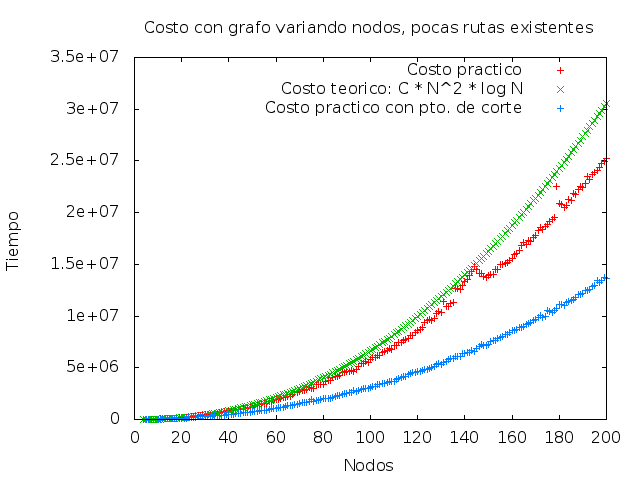
\includegraphics[scale=0.6]{ej2-grafico1.png}
\end{figure}


\begin{figure}[H]
	\centering
	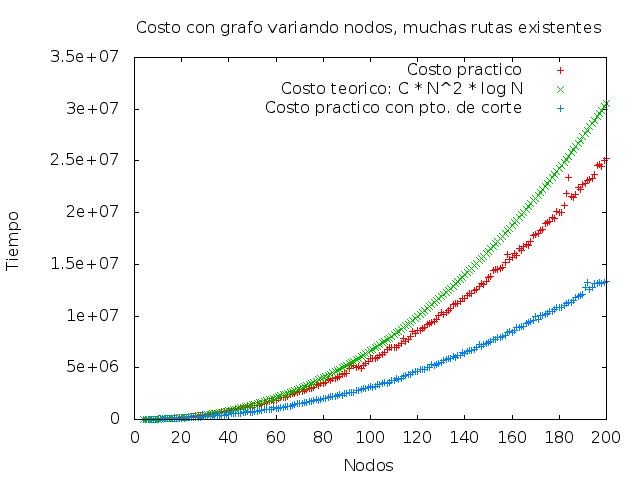
\includegraphics[scale=0.6]{ej2-grafico2.png}
\end{figure}


\subsection{Conclusiones}

